\chapter{Spring Data JPA}

\fcolorbox{black}[HTML]{E9F0E9}{\parbox{\textwidth}{%
\noindent \textbf{Learning goals}\\
The junior-colleague
\begin{enumerate}[nolistsep]
\item can describe the concept of ORM.
\item can explain what JPA is.
\item can list and describe different JPA providers.
\item can define what Hibernate is and its role within JPA.
\item can explain the benefits of using Spring Data JPA.
\item can describe what a persistence unit entails in JPA.
\item can outline and explain the fundamental interfaces of JPA.
\item can discuss what the persistence context is and its importance.
\item can implement and explain entity classes in JPA.
\item can use and explain the different annotations in JPA entity classes.
\item can describe the lifecycle of entity objects in JPA.
\item can implement and describe various types of relationships in entity classes.
\item can implement CRUD operations using JPA.
\item can implement queries using method names and annotations in Spring Data JPA.
\item can describe and implement transactions in JPA.
\item can explain transaction propagation.
\item can explain fetching strategy.
\item can describe and configure application properties for logging and debugging.
\item can describe and configure application properties for managing transactions.
\item can implement pagination and filtering in JPA applications.
\item can explain, identify, and solve the N + 1 query problem in JPA applications.
\end{enumerate}}}

  
\section{What is ORM?}

Object-Relational Mapping (ORM) is a technique that lets you query and manipulate data from a relational database using an object-oriented programming language.

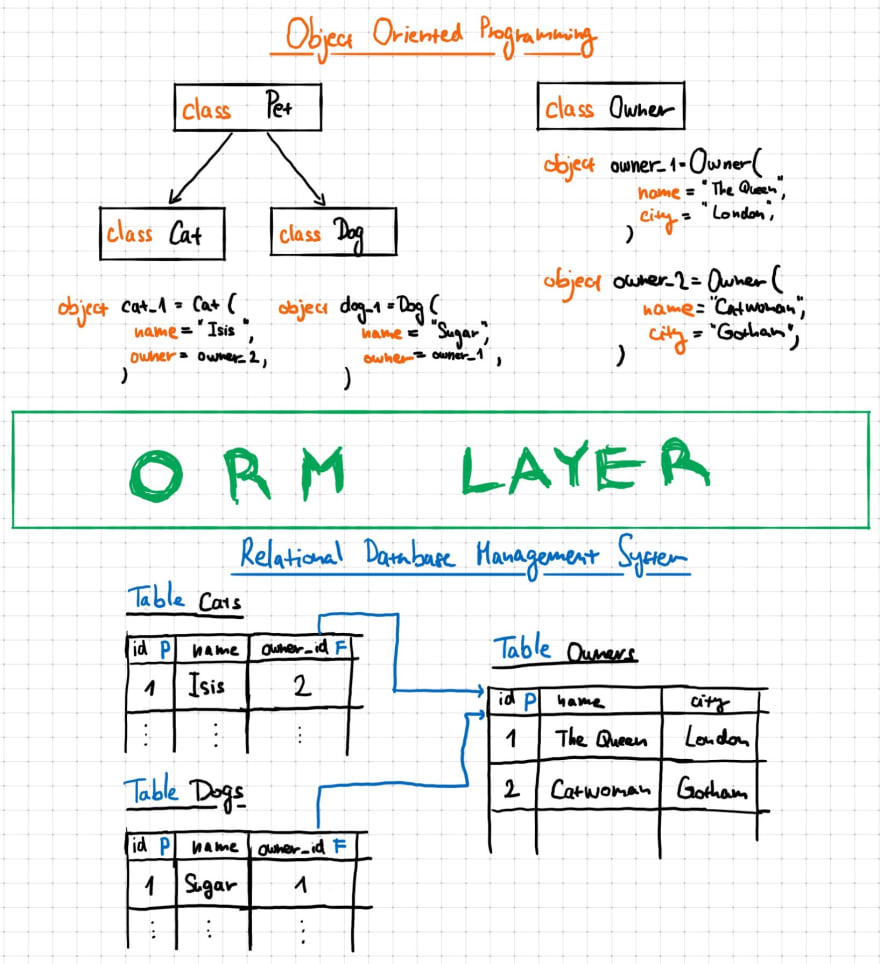
\includegraphics[width=\textwidth]{./images/chapter6/orm}


\section{What is JPA?}

The Java Persistence API (or more correctly Jakarta Persistence API) is a specification that defines how to persist data in Java applications. JPA mainly focuses on the ORM layer and managing persistent objects.

JPA is a specification which means JPA consists of implementation guidelines for the Java ORM layer and the syntax. The specification only comes with interfaces, no actual implementation.  A reference implementation can be provided but other companies can create and distribute their own implementation of the specification.

\frame{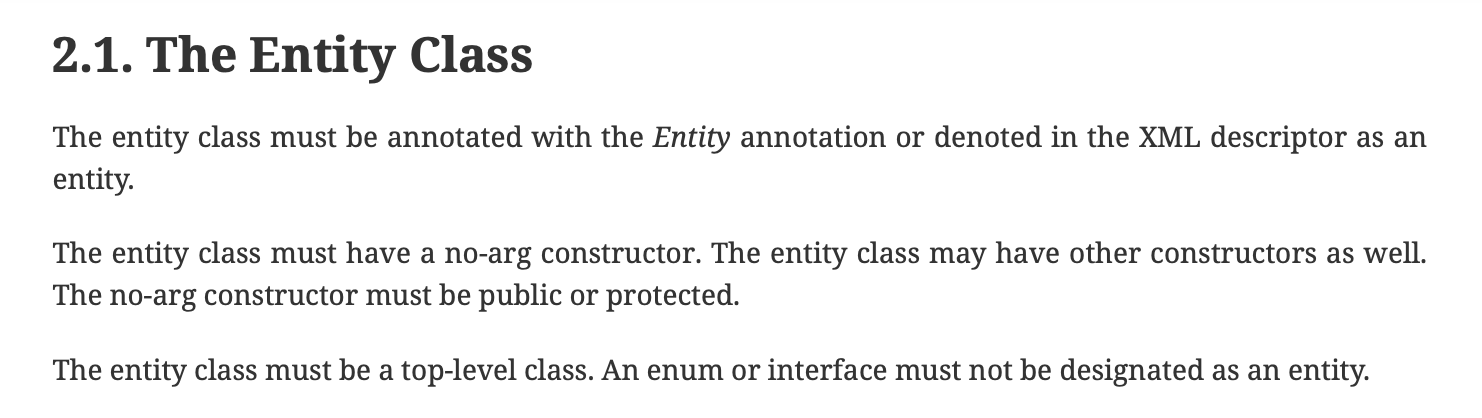
\includegraphics[width=\textwidth]{./images/chapter6/entity_class_specification}}

Hibernate is the default JPA provider when building Spring Boot applications. \footnote{\url{https://hibernate.org/ and https://hibernate.org/orm/}}.  

Spring Data JPA is a part of the larger Spring Data family, aimed at simplifying data access and manipulation across a variety of database technologies.
Spring Data JPA adds a layer on top of JPA. It uses all the features defined by the JPA specification, but adds no-code implementation of the repository pattern and the creation of database queries from method names.
Within this framework, JpaRepository is a key interface that extends Spring Data’s repository abstraction, specifically tailored for JPA technology. This interface is designed to streamline the storage and retrieval processes of entity instances, reducing the amount of boilerplate code developers need to write and offering a more intuitive interaction with the data layer.
JpaRepository extends PagingAndSortingRepository which in turn extends CrudRepository.

Their main functions are:

\begin{itemize}
\item CrudRepository mainly provides CRUD functions.
\item PagingAndSortingRepository provides methods to do pagination and sorting records.
\item JpaRepository provides some JPA-related methods such as flushing the persistence context and deleting records in a batch.
\end{itemize}


\section{Datasource and application properties}

In Spring Boot a DataSource-object is the preferred means of getting a connection to a database.
The interface jakarta.sql.DataSource is implemented by the database driver vendor. 

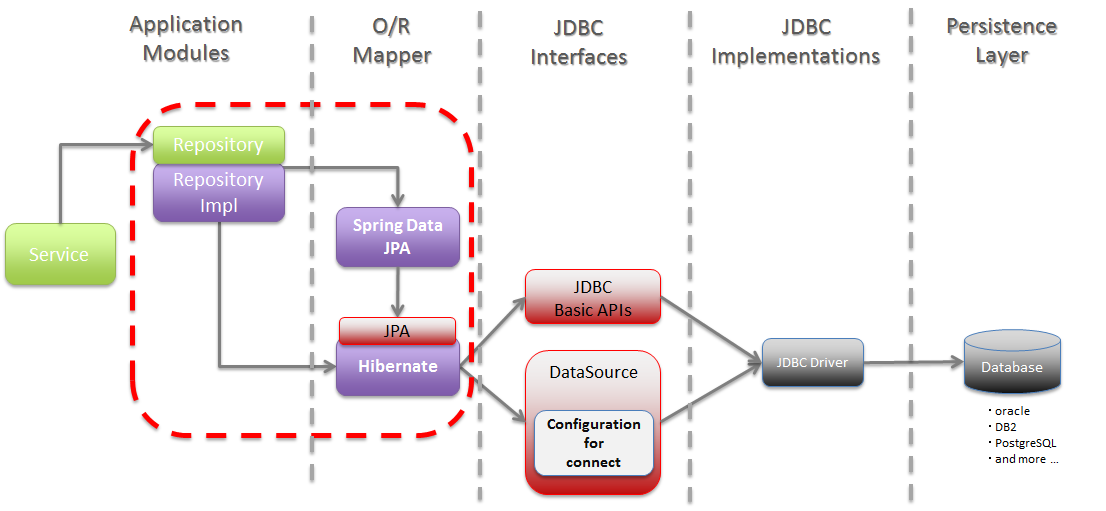
\includegraphics[width=\textwidth]{./images/chapter-jpa/springdatajpa}

The datasource can be specified in the application.properties file.
Here are some common database properties:

\begin{tabular}{|l|p{8cm}|}
\hline
spring.datasource.url & JDBC URL of the database.\\
spring.datasource.username & Login username of the database.\\
spring.datasource.password & Login password of the database.\\
spring.jpa.show-sql & Whether to enable logging of SQL statements. Default: false\\
spring.jpa.hibernate.ddl-auto & Possible values: none (production), create, create-drop, validate and update. \footnote{\url{https://stackoverflow.com/questions/42135114/how-does-spring-jpa-hibernate-ddl-auto-property-exactly-work-in-spring}}\\
\hline
\end{tabular}

Alternatively, the data source configuration can be done programmatically.

The appropriate JDBC driver for your database must be included in your project by declaring the driver as a dependency in your project's Maven configuration file, pom.xml. The dependency ensures that the JDBC driver is available during runtime, allowing Spring Data JPA to establish and manage database connections.

Here is an example of how to include a JDBC driver for MySQL in your pom.xml file:

\begin{lstlisting}
<dependency>
<groupId>com.mysql</groupId>
<artifactId>mysql-connector-j</artifactId>
<scope>runtime</scope>
</dependency>
\end{lstlisting}


Similarly,  to connect to a PostgreSQL database, you would use the PostgreSQL JDBC driver as shown below:

\begin{lstlisting}
<dependency>
<groupId>org.postgresql</groupId>
<artifactId>postgresql</artifactId>
<scope>runtime</scope>
</dependency>
\end{lstlisting}

Adjusting the driver version in your pom.xml may be necessary as you upgrade your database server or migrate to a newer version of Spring Data JPA.

\subsection{Application properties}

Configuring a Spring Boot application involves more than just setting up the datasource. In this section, we delve into application properties that assist in database initialization, enhance logging and debugging capabilities, and facilitate robust transaction management. Understanding these properties will enable you to fine-tune your application for better performance, easier maintenance, and more effective error handling.

\subsubsection{Database initialization}

The setting for Spring Data JPA's property \textit{spring.jpa.hibernate.ddl-auto} is directly transferred to Hibernate as the property \textit{hibernate.hbm2ddl.auto}. The permissible values — \textit{create}, \textit{create-drop}, \textit{validate}, and \textit{update} — determine how the schema tool management adjusts the database schema during application startup.


\subsubsection{Logging and debugging}

\textit{logging.level.ROOT} is used for configuring the base level of logging across all components in the application unless overridden.

\begin{itemize}
\item \textbf{spring.jpa.show-sql}: When set to true, Hibernate will log all SQL statements, which is invaluable for debugging and understanding how JPA translates entity operations into SQL.

\item \textbf{spring.jpa.properties.hibernate.format\_sql}: Improves the readability of the SQL logged by Hibernate by formatting it.

\item \textbf{logging.level.org.hibernate.type.descriptor.sql}: Adjusting the log level makes it possible to log JDBC parameters and the results coming from the database.
\end{itemize}



\subsubsection{Transaction Management}

Some properties are related to transaction management. 

Setting \textit{spring.datasource.hikari.auto-commit=false} applies to the HikariCP connection pool. Setting auto-commit to false means that each connection obtained from the pool will not automatically commit its transactions after each SQL statement. Instead, the application must explicitly call commit or rollback on the transaction. This setting is crucial for ensuring that the transaction management can be fully controlled by the application.

When setting \textit{spring.jpa.properties.hibernate.connection.autocommit} to false, Hibernate will not commit after each statement execution, allowing for transactional integrity where operations can be rolled back if a transaction is incomplete or encounters an error.

Finally, \textit{spring.jpa.open-in-view=false} controls whether a Hibernate Session is bound to the thread for the entire duration of a web request. Setting it to false avoids the anti-pattern where the database transaction is kept open during the view rendering, potentially leading to performance issues, such as longer database connection hold times and difficulties in detecting transactional issues early in the request processing. It is important to set this property to false. It may occur that your application works on the developer machine but fails under load.
Read the following article for additional information:
\url{https://backendhance.com/en/blog/2023/open-session-in-view/}


\section{The Entity class}

Let's explore an entity class that uses key annotations to manipulate event records in a database.

\begin{lstlisting}[frame=single,language=java]
import jakarta.persistence.Entity;
import jakarta.persistence.Table;
import jakarta.persistence.Column;
import jakarta.persistence.Id;
import jakarta.persistence.GeneratedValue;
import jakarta.persistence.GenerationType;
import jakarta.persistence.Embedded;
import jakarta.persistence.Embeddable;

@Entity
@Table(name = "events")
public class Event {

    @Id
    @GeneratedValue(strategy = GenerationType.IDENTITY)
    private Long id;

    @Column(name = "name", nullable = false,  length = 200)
    private String title;
    
    @Enumerated(value = EnumType.STRING)
    private Category category;

    @Embedded
    private EventDetails details;

    // Constructors, getters, and setters
}

@Embeddable
class EventDetails {
    private LocalDate date;
    @Column(length = 512)
    private String location;

    // Constructors, getters, and setters
}
\end{lstlisting}

A JPA entity class is a POJO (Plain Old Java Object) class  that is annotated as having the ability to represent objects in the database.
The \textbf{@Entity} annotation is used to declare that a class is an entity, so JPA will manage it and map it to a database table.

\textbf{@Table} specifies the table in the database with which the entity is mapped.

The \textbf{@Id} annotation marks a field as a primary key field.

The \textbf{@GeneratedValue} annotation is used to configure the primary key generation strategy for an entity. This annotation is usually combined with @Id to specify that the persistence provider should automatically generate a unique identifier for the entity objects. There are several strategies defined in the GenerationType enumeration that can be used with @GeneratedValue. Here's an overview:

\begin{itemize}
\item \textbf{GenerationType.AUTO}

This is the default strategy and the persistence provider will choose the generation strategy based on the specific database capabilities and dialect. 

\item \textbf{GenerationType.IDENTITY}

Indicates that the persistence provider must assign primary keys using the database identity column. This is typically supported by SQL databases with an auto-increment column.

\item \textbf{GenerationType.SEQUENCE}

Specifies that the primary key values will be generated using a database sequence. This is a special database object that generates numbers in sequential order. Not all databases support sequences.
This strategy is useful for databases supporting sequences, like Oracle, PostgreSQL, etc. It's beneficial for high-volume applications due to better performance compared to IDENTITY, as the sequence generation can be more efficiently managed.

\item \textbf{GenerationType.TABLE}

Uses a database table to simulate a sequence. This strategy uses a table to hold the next id incrementally. It's a portable solution but not as efficient as using database-specific features like sequences or identity columns.
\end{itemize}

The \textbf{@Column} annotation is used to specify the details of the column to which a field or property will be mapped. You can use column annotation with the following most commonly used attributes:
\begin{itemize}
\item \textbf{name}: specify the name of the column.
\item \textbf{length}: specify the size of thee column, particularly for a String value.
\item \textbf{nullable}: mark the column to be NOT NULL when the database schema is generated.
\item \textbf{unique}: mark the column to contain only unique values.
\end{itemize}


The \textbf{@Embeddable} annotation marks a class to be embedded within another entity.
In this example,  the EventDetails does not need its own table; instead, its properties are incorporated into the table of the entity that embeds it.

The annotation \textbf{@Embedded}  is used to denote a class whose instances are stored as an intrinsic part of an owning entity.
 All the fields of EventDetails class are embedded within the events table, avoiding the need for a separate table.

The \textbf{@Enumerated} annotation is used to specify how an enum type should be mapped to a database column when using JPA. This annotation can take one of two values: EnumType.STRING or EnumType.ORDINAL.

Using EnumType.STRING as the value for the @Enumerated annotation means that the enum values are stored in the database as their corresponding string names. This approach is often preferred because it makes the database values clear and readable, and it ensures that changes to the order of the enum values in the code do not affect the stored data.

\section{Entity lifecycle}

The EntityManager is a core interface of JPA.  An instance of EntityManager is used to create and remove  entity instances, to find entities by their primary key,  and to query over entities.  In fact,  an instance of the EntityManager is used to interact with the persistence context. 

The persistence context is one of the main concepts in JPA.
It is a set of all entity object that you are currently using or used recently. You can think of the persistence context as some kind of first-level cache. Each entity object in the persistence context represents a record in the database.
The persistence context manages these entity objects and their lifecycle. Each entity object has one of 4 states: new, managed, removed, and detached.

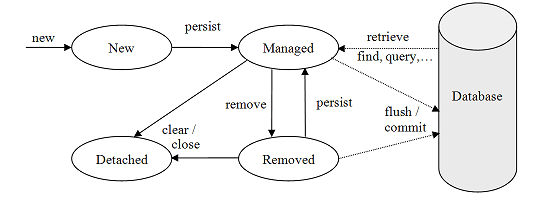
\includegraphics[width=\textwidth]{./images/chapter6/entity_states}

A newly instantiated entity object is in state \textbf{new} or \textbf{transient}. The entity object hasn't been persisted yet, so there's no database record yet. The persistence context does not know about the entity object yet. 

All entity objects that attached to the persistence context are in the lifecycle state \textbf{managed}. An entity object becomes managed when it is persisted to the database. Entity object retrieved from the database are also in the managed state.
If a managed entity object is modified (updated) within an active transaction, the change is detected by the persistence context and passed on to the database.

When a managed entity is removed within an active transaction, the state changes from managed to removed, and the record is physically deleted from the database (when the transaction commits).

An entity gets detached when it is no longer managed by the persistence context but still represents a record in the database.
Detached objects are limited in functionality.

 
Programmatically we need to use the entitymanager to change the state of the entity object in the persistence context which results in changes or updates in our database. 

When using Spring Data JPA you don't have to implement the interaction with the entitymanager. When you create a Repository, the SimpleJpaRepository class provided by Spring Data JPA provides the default implementation. SimpleJpaRepository class internally uses JPA entitymanager.

\begin{oefening}
Open the class SimpleJpaRepository and take a look at its implementation (e.g. save()-method).
\end{oefening}


\section{Relationships}

\subsection{OneToOne relationship}

A OneToOne relationship in JPA is used when one entity instance is associated with exactly one instance of another entity.  In this example a user has exactly one passport.

In a \textbf{uni-directional} OneToOne relationship, only one side of the relationship maintains knowledge of the other side’s existence. Consider a scenario where each Person has exactly one Passport. The Person entity holds a reference to the Passport, but the Passport does not hold any reference to the Person.

\begin{lstlisting}
@Entity
public class Person {
    @Id
    @GeneratedValue(strategy = GenerationType.IDENTITY)
    private Long id;
    
    @OneToOne(cascade = CascadeType.ALL)
    @JoinColumn(name = "passport_id", referencedColumnName = "id")
    private Passport passport;

    // Standard getters and setters
}

@Entity
public class Passport {
    @Id
    @GeneratedValue(strategy = GenerationType.IDENTITY)
    private Long id;
    
    private String number;

    // Standard getters and setters
}
\end{lstlisting}

In this example, the Person entity contains a Passport field annotated with @OneToOne. The @JoinColumn annotation specifies the column in the Person table that joins to the primary key of the Passport entity.

The concept of \"cascade types\" defines how persistence operations such as save, delete, and update performed on one entity should be propagated (or cascaded) to its associated entity. 

When using the @OneToOne annotation in JPA, you can specify a cascade type to automate the persistence lifecycle management of the associated entity. Here are the most common cascade types used in JPA:

\begin{itemize}
\item \textbf{CascadeType.PERSIST}: When persisting an entity, also persist the associated entity.  For example, when saving a Person object, also save its associated Passport.

\item \textbf{CascadeType.MERGE}: When merging the state of an entity into the current persistence context, also merge the entity held in this field.

\item \textbf{CascadeType.REMOVE}: When deleting an entity, also delete the associated entity. This is particularly useful when the associated entity no longer makes sense to exist independently.

\item \textbf{CascadeType.REFRESH}: When refreshing an entity, also refresh the entities held in this field. This means reloading the content of the associated entity from the database, which can be useful if the database might be changed by other processes.

\item \textbf{CascadeType.DETACH}: When an entity is detached from the persistence context, also detach the entities held in this field.

\item \textbf{CascadeType.ALL}: A convenience that cascades all the above operations (PERSIST, MERGE, REMOVE, REFRESH, DETACH). Using CascadeType.ALL is common for @OneToOne and @OneToMany associations.
\end{itemize}

In a \textbf{bi-directional} OneToOne relationship, both entities are aware of each other. This relationship allows navigation from either side. Using the same example as above, both the Person and Passport entities can have references to each other.

\begin{lstlisting}
@Entity
public class Person {
    @Id
    @GeneratedValue(strategy = GenerationType.IDENTITY)
    private Long id;

    @OneToOne(mappedBy = "person", cascade = CascadeType.ALL)
    private Passport passport;

    // Standard getters and setters
}

@Entity
public class Passport {
    @Id
    @GeneratedValue(strategy = GenerationType.IDENTITY)
    private Long id;

    private String number;

    @OneToOne
    @JoinColumn(name = "person_id")
    private Person person;

    // Standard getters and setters
}
\end{lstlisting}

In this bi-directional setup, the Person entity uses the mappedBy attribute in the @OneToOne annotation to indicate that the Person is not the owner of the relationship and that the Passport entity contains the foreign key.

\subsection{ManyToOne relationship}

A ManyToOne relationship in JPA is commonly used when one entity is related to multiple instances of another entity. For instance, in a blog system, many posts may belong to one category.

Uni-directional ManyToOne Relationship
In a uni-directional ManyToOne relationship, only the 'many' side of the relationship is aware of the 'one' side. This setup is often seen when the 'one' side doesn't need to directly access the 'many' side.

Example: Books and Authors
Suppose each book can have one author, but each author can write many books. Here, the relationship from books to authors is a typical example of a uni-directional ManyToOne relationship.

\begin{lstlisting}
@Entity
public class Book {
    @Id
    @GeneratedValue(strategy = GenerationType.IDENTITY)
    private Long id;

    private String title;

    @ManyToOne
    @JoinColumn(name = "author_id", nullable = false)
    private Author author;

    // Standard getters and setters
}

@Entity
public class Author {
    @Id
    @GeneratedValue(strategy = GenerationType.IDENTITY)
    private Long id;

    private String name;

    // Standard getters and setters, no reference back to Book
}
\end{lstlisting}

In this model, each Book entity holds a reference to its Author, which is annotated with @ManyToOne. The @JoinColumn annotation specifies the foreign key column in the Book table that links to the Author.

Repository Configuration
Repositories for each entity can be defined as follows:

\begin{lstlisting}
public interface BookRepository extends JpaRepository<Book, Long> {
}

public interface AuthorRepository extends JpaRepository<Author, Long> {
}
\end{lstlisting}

Bi-directional ManyToOne Relationship
In a bi-directional relationship, both sides of the relationship are aware of each other. This is useful when you want to navigate the relationship from either side.

Example: Books and Authors Continued
Expanding on the previous example, suppose now we want authors to also be aware of the books they've written.

Entity Definition
\begin{lstlisting}
@Entity
public class Book {
    @Id
    @GeneratedValue(strategy = GenerationType.IDENTITY)
    private Long id;

    private String title;

    @ManyToOne
    @JoinColumn(name = "author_id", nullable = false)
    private Author author;

    // Standard getters and setters
}

@Entity
public class Author {
    @Id
    @GeneratedValue(strategy = GenerationType.IDENTITY)
    private Long id;

    private String name;

    @OneToMany(mappedBy = "author")
    private Set<Book> books = new HashSet<>();

    // Standard getters and setters
}
\end{lstlisting}

In this bi-directional setup, the Author class includes a Set<Book> to hold the collection of books. The @OneToMany annotation in Author uses the mappedBy attribute to indicate that the Author entity is not the owner of the relationship and that the Book entity contains the foreign key.

\subsection{ManyToMany relationship}


A ManyToMany relationship is used when multiple instances of one entity are associated with multiple instances of another entity. Using the example of books and authors, a ManyToMany relationship would be appropriate if each book could have multiple authors and each author could write multiple books. 

In a uni-directional ManyToMany relationship, only one entity maintains the relationship information.

Imagine a scenario where each book can have multiple authors, but we are only interested in navigating from books to authors and not the other way around.

\begin{lstlisting}
@Entity
public class Book {
    @Id
    @GeneratedValue(strategy = GenerationType.IDENTITY)
    private Long id;

    private String title;

    @ManyToMany
    @JoinTable(
        name = "book_author",
        joinColumns = @JoinColumn(name = "book_id"),
        inverseJoinColumns = @JoinColumn(name = "author_id")
    )
    private Set<Author> authors = new HashSet<>();

    // Standard getters and setters
}

@Entity
public class Author {
    @Id
    @GeneratedValue(strategy = GenerationType.IDENTITY)
    private Long id;

    private String name;

    // Standard getters and setters, no reference back to Books
}
\end{lstlisting}
In this example, the Book entity defines a ManyToMany relationship to the Author entity. The @JoinTable annotation specifies the table that maps books to authors, including columns for each foreign key.


In a bi-directional ManyToMany relationship, both entities are aware of each other, and navigation is possible from either side.

This time, both books and authors are aware of each other and can navigate the relationship.

\begin{lstlisting}
@Entity
public class Book {
    @Id
    @GeneratedValue(strategy = GenerationType.IDENTITY)
    private Long id;

    private String title;

    @ManyToMany
    @JoinTable(
        name = "book_author",
        joinColumns = @JoinColumn(name = "book_id"),
        inverseJoinColumns = @JoinColumn(name = "author_id")
    )
    private Set<Author> authors = new HashSet<>();

    // Standard getters and setters
}

@Entity
public class Author {
    @Id
    @GeneratedValue(strategy = GenerationType.IDENTITY)
    private Long id;

    private String name;

    @ManyToMany(mappedBy = "authors")
    private Set<Book> books = new HashSet<>();

    // Standard getters and setters
}
\end{lstlisting}

In the bi-directional arrangement, the Author entity includes a Set<Book> to hold the collection of books. The mappedBy attribute indicates that the Author is not the owner of the relationship, and the mapping details are managed by the Book entity.

\section{Fetching strategy}

JPA provides two main fetching strategies to control how related entities are loaded from the database:

\begin{itemize}
\item \textbf{Eager Fetching}: With eager fetching, related entities are loaded immediately with the main entity, whether they are accessed in the application or not. This can lead to performance issues if the relationships involve large sets of data. Eager fetching is often used when the data sets are small or always used together with the main entity.

\item \textbf{Lazy Fetching}: Lazy fetching loads the related entities only when they are explicitly accessed in the application. This can improve performance by reducing the initial load time and the amount of memory consumed. However, it requires careful management of the persistence context to avoid LazyInitializationException.
\end{itemize}

In the case of ManyToMany relationships, the default fetching strategy is lazy because eager fetching can result in very large numbers of joins and thus severe performance degradation.

\begin{lstlisting}
@ManyToMany(fetch = FetchType.LAZY)
private Set<Author> authors = new HashSet<>();
\end{lstlisting} 

Understanding and choosing the right fetching strategy based on the specific use case and data access patterns is crucial for developing efficient, scalable applications.

Consider the following method findBooksByAuthor() in a BookService.
When we look closely at the logging of the SQL-queries. We see that first, the author is retrieved and later, the author's books are retrieved on the moment we call author.getBooks(), not sooner. This is lazy loading or lazy fetching. When dealing with one-to-many or many-to-many relationships, lazy fetching is mostly the best solution in terms of performance.

Make sure your method is running in  a transaction. Otherwise you will encounter a LazyInitializationException.
\begin{verbatim}
org.hibernate.LazyInitializationException: 
failed to lazily initialize a collection of role: be.pxl.domain.Author.books:
could not initialize proxy - no Session
\end{verbatim}

\begin{lstlisting}
@Service
public class BookService {

    private static final Logger LOGGER = LogManager.getLogger(BookService.class);

    private final AuthorRepository authorRepository;

    public BookService(AuthorRepository authorRepository) {
        this.authorRepository = authorRepository;
    }

    @Transactional
    public List<String> getBooksByAuthor(String authorName) {
        LOGGER.info("Starting getBooksByAuthor");
        Author author = authorRepository.findAuthorByName(authorName).orElseThrow(() -> new NotFoundException(""));
        LOGGER.info("Author retrieved...");
        return author.getBooks().stream().map(Book::getTitle).toList();
    }
}
\end{lstlisting}

\begin{verbatim}
2024-04-23T20:23:48.883+02:00  INFO 26656 --- [nio-8080-exec-8]
be.pxl.service.BookService      : Starting getBooksByAuthor
Hibernate: 
    select
        a1_0.id,
        a1_0.name 
    from
        authors a1_0 
    where
        a1_0.name=?
2024-04-23T20:23:48.946+02:00  INFO 26656 --- [nio-8080-exec-8]
be.pxl.service.BookService      : Author retrieved...
Hibernate: 
    select
        b1_0.author_id,
        b1_1.id,
        b1_1.title 
    from
        book_authors b1_0 
    join
        books b1_1 
            on b1_1.id=b1_0.book_id 
    where
        b1_0.author_id=?
\end{verbatim}

If we change the relationship between Author and Books to eager fetching, the books are retrieved on the moment we search the author by its name.


\begin{lstlisting}
@Entity
@Table(name = "authors")
public class Author {
    @Id
    @GeneratedValue(strategy = GenerationType.IDENTITY)
    private Long id;

    private String name;

    @ManyToMany(mappedBy = "authors", fetch = FetchType.EAGER)
    private Set<Book> books = new HashSet<>();

    // Standard getters and setters

    public void addBook(Book book) {
        books.add(book);
    }

    public Set<Book> getBooks() {
        return books;
    }
}
\end{lstlisting}

\begin{verbatim}
2024-04-23T20:21:02.145+02:00  INFO 19956 --- [nio-8080-exec-6]
be.pxl.service.BookService      : Starting getBooksByAuthor
Hibernate: 
    select
        a1_0.id,
        a1_0.name 
    from
        authors a1_0 
    where
        a1_0.name=?
Hibernate: 
    select
        b1_0.author_id,
        b1_1.id,
        b1_1.title 
    from
        book_authors b1_0 
    join
        books b1_1 
            on b1_1.id=b1_0.book_id 
    where
        b1_0.author_id=?
2024-04-23T20:21:02.216+02:00  INFO 19956 --- [nio-8080-exec-6]
be.pxl.service.BookService      : Author retrieved...
\end{verbatim}

Always be very carefull with bi-directional relationships and eager fetching. The performance cost may be underestimated. In this case, if an author has written many books, it may be beneficial, to only maintain the owning part of the relationship and search for in author's books with a query in the BookRepository.

\section{Transactions}

The \textbf{@Transactional} annotation in Spring Boot is used to declare that a method or a class should be executed within a transactional context.

A transaction is a sequence of actions that are treated as a single unit of work. These actions should either complete entirely or take no effect at all.
Transaction Management ensures that an application maintains data integrity and consistency in scenarios involving multiple transaction operations.

Newly created entities should always be saved to the database, however changes to managed entities are persisted automatically when the transaction is committed.

\subsection{Usage of @Transactional}

When placed above a method, @Transactional ensures the method executes within a transaction. If a transaction is already running, the method by default runs within that transaction.

If @Transactional is placed at the class level, it applies to all the public methods of that class.


Transaction propagation behaviour defines how transactions relate to each other. Common propagation types include:

\begin{itemize}
\item REQUIRED: Use the current transaction or start a new one if none exists.
\item REQUIRES\_NEW: Always start a new transaction, suspending the current one if it exists.
\item SUPPORTS: Run within the current transaction if it exists; otherwise, run non-transactionally.
\item NEVER: Ensure no current transaction exists, throwing an exception if one exists.
\end{itemize}


Suppose a method annotated with @Transactional is called in a Spring Boot application. The transaction manager checks if a current transaction exists. Depending on the propagation setting:
\begin{itemize}
\item The current transaction is used, or a new transaction is created.
\item The current transaction is suspended, and a new transaction is created.
\end{itemize}
Then the method executes and database operations are performed as part of the current transaction.
If the method completes successfully, the transaction is committed.
If an exception occurs, the transaction is rolled back.

Let’s consider an example with Book and Author entities. We want to ensure that adding a book linked to an author is transactional (either both the book and the author are saved, or neither).

\begin{lstlisting}
@Entity
public class Author {
    @Id
    @GeneratedValue(strategy = GenerationType.AUTO)
    private Long id;
    private String name;
    // constructors, getters, and setters
}

@Entity
public class Book {
    @Id
    @GeneratedValue(strategy = GenerationType.AUTO)
    private Long id;
    private String title;
    @ManyToOne
    private Author author;
    // constructors, getters, and setters
}

@Service
public class BookService {
    @Autowired
    private BookRepository bookRepository;
    @Autowired
    private AuthorRepository authorRepository;

    @Transactional
    public void addBookAndAuthor(Book book, Author author) {
        authorRepository.save(author); // Save author
        book.setAuthor(author);
        bookRepository.save(book); // Save book
        // Both saves are part of the same transaction
    }
}
\end{lstlisting}

\subsection{Transaction propagation}

In the context of transaction management, transaction propagation behaviours define how transactions are handled when one transactional method calls another. The common types of transaction propagation behaviours with are:
\begin{itemize}
\item \textbf{REQUIRED} - Use the existing transaction if available; start a new one if none exists. This is the default value.
\item \textbf{SUPPORTS} - Execute within the existing transaction if one is already present; execute non-transactionally if there is no transaction.
\item \textbf{MANDATORY} - Require an existing transaction; throw an exception if there is no existing transaction.
\item \textbf{REQUIRES\_NEW} - Suspend the current transaction if one exists, and start a new transaction.
\item \textbf{NOT\_SUPPORTED} - Suspend the existing transaction and execute non-transactionally.
\item \textbf{NEVER} - Execute non-transactionally; throw an exception if there is an existing transaction.
\end{itemize}

We will discuss these transaction propagation behaviours with example code.

\begin{lstlisting}
public record JoinOrganisationDto(String organisation, String employee) {
}

@RestController
@RequestMapping("/organisation")
public class OrganisationController {

    private final OrganisationService organisationService;

    public OrganisationController(OrganisationService organisationService) {
        this.organisationService = organisationService;
    }

    @PostMapping("/join")
    public void joinOrganisation(@RequestBody JoinOrganisationDto joinOrganisationDto) {
        organisationService.joinOrganisation(joinOrganisationDto.organisation(), joinOrganisationDto.employee());
    }
}

@Entity
public class Employee {
    @Id
    @GeneratedValue(strategy = GenerationType.IDENTITY)
    private Long id;
    @ManyToOne
    private Organisation organisation;


    private String name;

    public String getName() {
        return name;
    }

    public void setName(String name) {
        this.name = name;
    }

    public void setOrganisation(Organisation organisation) {
        this.organisation = organisation;
    }
}

@Entity
public class Organisation {
    @Id
    @GeneratedValue(strategy = GenerationType.IDENTITY)
    private Long id;
    private String name;

    public void setName(String name) {
        this.name = name;
    }

    public String getName() {
        return name;
    }
}

@Service
public class OrganisationService {

    private final OrganizationRepository organizationRepository;
    private final EmployeeService employeeService;


    public OrganisationService(OrganizationRepository organizationRepository, EmployeeService employeeService) {
        this.organizationRepository = organizationRepository;
        this.employeeService = employeeService;
    }

    public void joinOrganisation(String organisationName, String employeeName) {
        Organisation organisation = organizationRepository.findByName(organisationName).orElseThrow(() -> new NotFoundException("Not found"));
        Employee employee = employeeService.insertEmployee(employeeName);
        employee.setOrganisation(organisation);
    }
}

@Service
public class EmployeeService {

    public Employee insertEmployee(String name) {
        Employee employee = new Employee();
        employee.setName(name);
        employee = employeeRepository.save(employee);
        return employee;
    }
}

public interface OrganizationRepository extends JpaRepository<Organisation, Long> {
    Optional<Organisation> findByName(String name);
}

\end{lstlisting}

\begin{verbatim}
POST http://localhost:8080/organisations/join
{
	"organisation" : "Happy Organisation",
	"employee": "Tamara"
}
\end{verbatim}

The employee data is persisted, but when something goes wrong in the method joinOrganisation, we end up with inconsistent data. The employee is saved without an organisation.

\begin{lstlisting}
 public Employee insertEmployee(String name) {
        Employee employee = new Employee();
        employee.setName(name);
        employee = employeeRepository.save(employee);
        return employee;
}

public void joinOrganisation(String organisationName, String employeeName) {
        Organisation organisation = organizationRepository.findByName(organisationName).orElseThrow(() -> new NotFoundException("Not found"));
        Employee employee = employeeService.insertEmployee(employeeName);
        employee.setOrganisation(organisation);
        throw new RuntimeException("Intentional error");
}
\end{lstlisting}

\subsubsection{Propagation.REQUIRED}

Let's add transaction management and discuss transaction propagation.
When you use the annotation @Transactional, the default value for transaction propagation is REQUIRED: @Transactional(propagation = Propagation.REQUIRED).

\begin{lstlisting}
@Transactional(propagation = Propagation.REQUIRED)
public void joinOrganisation(String organisationName, String employeeName) {
        Organisation organisation = organizationRepository.findByName(organisationName).orElseThrow(() -> new NotFoundException("Not found"));
        Employee employee = employeeService.insertEmployee(employeeName);
        employee.setOrganisation(organisation);
        //throw new RuntimeException("Intentional error");
}

@Transactional(propagation = Propagation.REQUIRED)
 public Employee insertEmployee(String name) {
        Employee employee = new Employee();
        employee.setName(name);
        employee = employeeRepository.save(employee);
        return employee;
}
\end{lstlisting}

When calling joinOrganisation a new transaction is created. This transaction is used when calling the method insertEmployee. This results in persisting an employee with his/her organisation. If an error occurs, the transaction is rolled back, and the employee is not persisted in the database. 

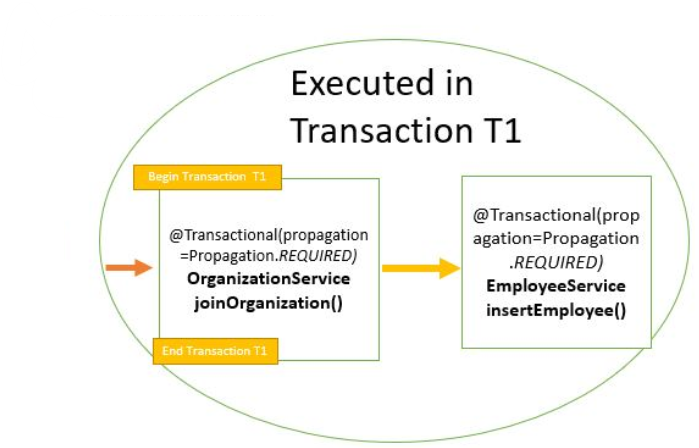
\includegraphics[width=8cm]{./images/chapter-jpa/transaction_propagation_1}


\subsubsection{Propagation.SUPPORTS}

\begin{lstlisting}
@Transactional(propagation = Propagation.REQUIRED)
public void joinOrganisation(String organisationName, String employeeName) {
        Organisation organisation = organizationRepository.findByName(organisationName).orElseThrow(() -> new NotFoundException("Not found"));
        Employee employee = employeeService.insertEmployee(employeeName);
        employee.setOrganisation(organisation);
        //throw new RuntimeException("Intentional error");
}

@Transactional(propagation = Propagation.SUPPORTS)
 public Employee insertEmployee(String name) {
        Employee employee = new Employee();
        employee.setName(name);
        employee = employeeRepository.save(employee);
        return employee;
}
\end{lstlisting}

The method insertEmployee uses the transaction that is created when calling the joinOrganisation method. However, if the insertEmployee is called directly from the controller, no transaction will be created.

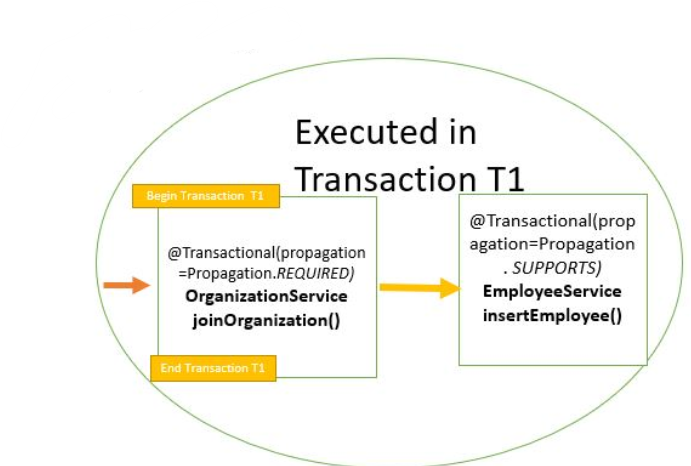
\includegraphics[width=8cm]{./images/chapter-jpa/transaction_propagation_2}

\subsubsection{Propagation.NOT\_SUPPORTED}

\begin{lstlisting}
@Transactional(propagation = Propagation.REQUIRED)
public void joinOrganisation(String organisationName, String employeeName) {
        Organisation organisation = organizationRepository.findByName(organisationName).orElseThrow(() -> new NotFoundException("Not found"));
        Employee employee = employeeService.insertEmployee(employeeName);
        employee.setOrganisation(organisation);
        //throw new RuntimeException("Intentional error");
}

@Transactional(propagation = Propagation.NOT_SUPPORTED)
 public Employee insertEmployee(String name) {
        Employee employee = new Employee();
        employee.setName(name);
        employee = employeeRepository.save(employee);
        return employee;
}
\end{lstlisting}

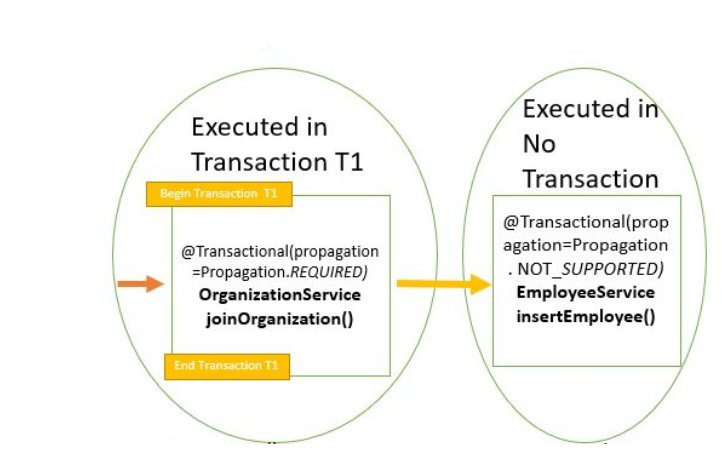
\includegraphics[width=8cm]{./images/chapter-jpa/transaction_propagation_3}

The method insertEmployee runs without transaction. It doesn't use the existing transaction, nor creates a new transaction. The employee is persisted in the database, without a link to its organisation.

\subsubsection{Propagation.REQUIRES\_NEW}

\begin{lstlisting}
@Transactional(propagation = Propagation.REQUIRED)
public void joinOrganisation(String organisationName, String employeeName) {
        Organisation organisation = organizationRepository.findByName(organisationName).orElseThrow(() -> new NotFoundException("Not found"));
        Employee employee = employeeService.insertEmployee(employeeName);
        employee.setOrganisation(organisation);
        //throw new RuntimeException("Intentional error");
}

@Transactional(propagation = Propagation.REQUIRES_NEW)
 public Employee insertEmployee(String name) {
        Employee employee = new Employee();
        employee.setName(name);
        employee = employeeRepository.save(employee);
        return employee;
}
\end{lstlisting}

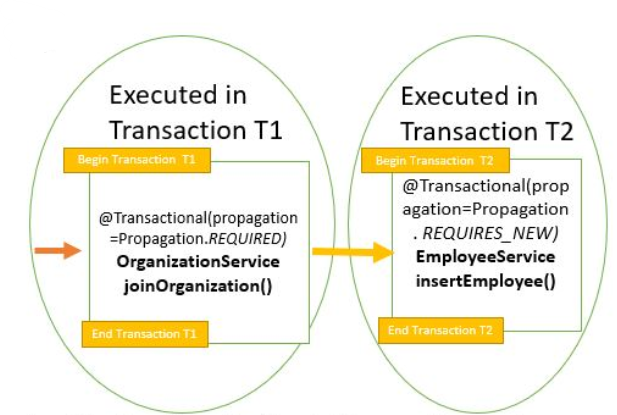
\includegraphics[width=8cm]{./images/chapter-jpa/transaction_propagation_4}

The method insertEmployee runs in its own, newly created transaction. If something goes wrong in the method joinOrganisation, only the sql statements from its own transaction are rolled back. Persisting the employee was already committed and will therefore not rollback.

\subsubsection{Propagation.NEVER}

\begin{lstlisting}
@Transactional(propagation = Propagation.REQUIRED)
public void joinOrganisation(String organisationName, String employeeName) {
        Organisation organisation = organizationRepository.findByName(organisationName).orElseThrow(() -> new NotFoundException("Not found"));
        Employee employee = employeeService.insertEmployee(employeeName);
        employee.setOrganisation(organisation);
        //throw new RuntimeException("Intentional error");
}

@Transactional(propagation = Propagation.NEVER)
 public Employee insertEmployee(String name) {
        Employee employee = new Employee();
        employee.setName(name);
        employee = employeeRepository.save(employee);
        return employee;
}
\end{lstlisting}

The method insertEmployee never runs in a transaction. If the calling method
runs in a transaction, an exception will occur.

\begin{verbatim}
org.springframework.transaction.IllegalTransactionStateException: Existing transaction found for transaction marked with propagation 'never'
\end{verbatim}

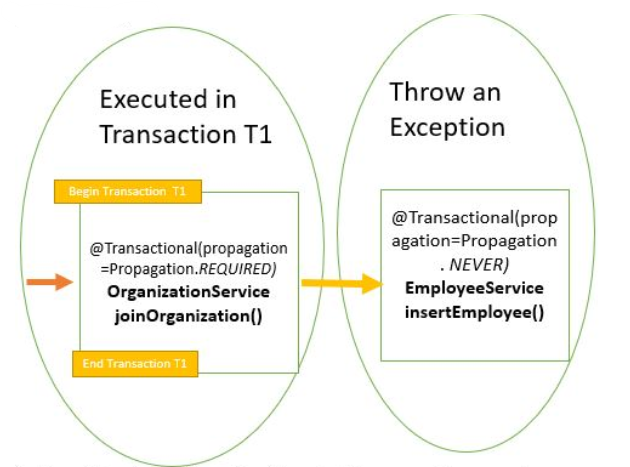
\includegraphics[width=8cm]{./images/chapter-jpa/transaction_propagation_5}

\subsubsection{Propagation.MANDATORY}

\begin{lstlisting}
@Transactional(propagation = Propagation.REQUIRED)
public void joinOrganisation(String organisationName, String employeeName) {
        Organisation organisation = organizationRepository.findByName(organisationName).orElseThrow(() -> new NotFoundException("Not found"));
        Employee employee = employeeService.insertEmployee(employeeName);
        employee.setOrganisation(organisation);
        //throw new RuntimeException("Intentional error");
}

@Transactional(propagation = Propagation.MANDATORY)
 public Employee insertEmployee(String name) {
        Employee employee = new Employee();
        employee.setName(name);
        employee = employeeRepository.save(employee);
        return employee;
}
\end{lstlisting}

The method insertEmployee uses the existing transaction.

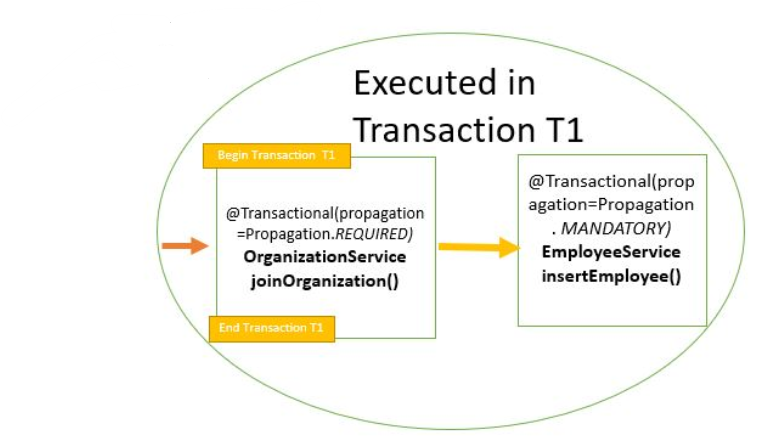
\includegraphics[width=8cm]{./images/chapter-jpa/transaction_propagation_6}

 If there is no current transaction that can be used, an error will be thrown. 

\begin{verbatim}
org.springframework.transaction.IllegalTransactionStateException: No existing transaction found for transaction marked with propagation 'mandatory'
\end{verbatim}

\section{Queries}

Basic CRUD queries are in Spring Data JPA available in the repositories. But there are multiple ways of creating custom queries in a Spring boot application. Let's discuss the different types of queries.

\subsection{Query methods}

Spring Data JPA can create queries based on method names. You can use keywords like \textit{findBy}, \textit{findAllBy},
\textit{findBy...And...}, ...

An overview of the keywords can be found in spring documentation \url{https://docs.spring.io/spring-data/jpa/reference/jpa/query-methods.html}.

\begin{lstlisting}
public interface ProductRepository extends JpaRepository<Product, Long> {
    // Query method with parameters for finding products by name and price
    List<Product> findByNameAndPrice(String name, double price);
}
\end{lstlisting}

\subsection{JPQL queries}

JPQL, or Java Persistence Query Language, is a query language designed to abstract database details from the developer, allowing queries to be written based on entity model classes rather than on database tables.


\begin{lstlisting}
public interface UserRepository extends JpaRepository<User, Long> {
    @Query("SELECT u FROM User u WHERE u.age >= :minAge")
    List<User> findByAgeGreaterThan(@Param("minAge") int minAge);
}
\end{lstlisting}

\subsection{Native SQL queries}

\begin{lstlisting}
public interface UserRepository extends JpaRepository<User, Long> {
    @Query(value = "SELECT * FROM users WHERE age >= :minAge", nativeQuery = true)
    List<User> findByAgeGreaterThanOrEqualNative(@Param("minAge") int minAge);
}
\end{lstlisting}


\section{Unit testing a repository}

Spring Data JPA offers an annotation @DataJpaTest which makes repository testing possible with a minimum of configuration. 

Add the h2 dependency with scope test in your pom.xml. This way the unit test for your repository will use the h2 database to test your queries.

\begin{lstlisting}
<dependency>
	<groupId>com.h2database</groupId>
	<artifactId>h2</artifactId>
	<scope>test</scope>
</dependency>
\end{lstlisting}

The builder pattern is used in this example to create entity objects for testing purpose. These entity objects are stored in the in-memory database. There is an IntelliJ IDEA plugin that generates the builder-classes for you (Generate Builder plugin).

\begin{lstlisting}
public final class AuthorBuilder {
    private String name;
    private Set<Book> books;

    private AuthorBuilder() {
    }

    public static AuthorBuilder anAuthor() {
        return new AuthorBuilder();
    }

    public AuthorBuilder withName(String name) {
        this.name = name;
        return this;
    }

    public AuthorBuilder withBooks(Set<Book> books) {
        this.books = books;
        return this;
    }

    public Author build() {
        Author author = new Author();
        author.setName(name);
        author.setBooks(books);
        return author;
    }
}
\end{lstlisting}

The @DataJpaTest annotation is used to test JPA repositories in Spring Boot applications. It’s a specialized test annotation that provides a minimal Spring context for testing the persistence layer. 

By default, each test method annotated with @DataJpaTest runs within a transactional boundary. This ensures that changes made to the database are automatically rolled back at the end of the test, leaving a clean slate for the next test.

The test class uses the entity managers, which is injected in the test with the @PersistenceContext annotation. The flush() forces to synchronize the persistence context to the database. The clear() empties the persistence context. Therefore, all entities are detached and can be fetched from the database.


\begin{lstlisting}[frame=single, language=java]
package be.pxl.repository;

import be.pxl.builder.AuthorBuilder;
import be.pxl.domain.Author;
import jakarta.persistence.EntityManager;
import jakarta.persistence.PersistenceContext;
import org.junit.jupiter.api.BeforeEach;
import org.junit.jupiter.api.Test;
import org.springframework.beans.factory.annotation.Autowired;
import org.springframework.boot.test.autoconfigure.orm.jpa.DataJpaTest;

import java.util.Arrays;
import java.util.Optional;

import static org.junit.jupiter.api.Assertions.assertEquals;
import static org.junit.jupiter.api.Assertions.assertTrue;

@DataJpaTest
public class AuthorRepositoryTest {

	@PersistenceContext
	protected EntityManager entityManager;

	@Autowired
	private AuthorRepository authorRepository;

	private final Author author1 = AuthorBuilder.anAuthor().withName("Famous Author").build();


	private final Author author2 = AuthorBuilder.anAuthor().withName("Not So Famous Author").build();

	@BeforeEach
	public void init() {
		authorRepository.saveAll(Arrays.asList(author1, author2));
		entityManager.flush();
		entityManager.clear();
	}

	@Test
	public void returnsAuthorByName() {
		Optional<Author> author = authorRepository.findAuthorByName("Famous Author");

		assertTrue(author.isPresent());
		assertEquals("Famous Author", author.get().getName());
	}

	@Test
	public void returnsEmptyOptionalWhenNoAuthorPlayerWithName() {
		Optional<Author> author = authorRepository.findAuthorByName("Bestseller Author");

		assertTrue(author.isEmpty());
	}
}
\end{lstlisting}


\section{Pagination}

Pageable is an interface provided by Spring Data that contains information about the pagination and sorting of data. It helps in structuring the way data is retrieved from the database in manageable chunks or pages, rather than pulling large quantities of data all at once, which can be inefficient and slow.


\begin{lstlisting}
@RestController
@RequestMapping("books")
public class BookController {

    private final BookService bookService;

    public BookController(BookService bookService) {
        this.bookService = bookService;
    }

    @GetMapping("search")
    public List<BookDto> searchBooks(@RequestBody FilterDto filter) {
        return bookService.searchBooks(filter);
    }

    @GetMapping
    public Page<BookDto> getBooks(Pageable pageable) {
        return bookService.findAllBooks(pageable);
    }
}
\end{lstlisting}

The parameter Pageable is automatically populated by Spring when the method is called. The Pageable object typically includes:
\begin{itemize}
\item page: The current page number (0-indexed, where 0 is the first page).
\item size: The number of records per page.
\item sort: Criteria for sorting the data (optional).
\end{itemize}

For example, a request URL might look like this: \textit{/books?page=0\&size=10\&sort=title,asc}. This tells the application to get the first page of books, with 10 books per page, sorted by title in ascending order.

\begin{lstlisting}
public interface BookRepository extends JpaRepository<Book, Long> {
}
\end{lstlisting}

\begin{lstlisting}
@Service
public class BookService {

    private static final Logger LOGGER = LogManager.getLogger(BookService.class);

    private final AuthorRepository authorRepository;
    private final BookRepository bookRepository;

    public BookService(AuthorRepository authorRepository, BookRepository bookRepository) {
        this.authorRepository = authorRepository;
        this.bookRepository = bookRepository;
    }

    public Page<BookDto> findAllBooks(Pageable pageable) {
        Page<Book> books = bookRepository.findAll(pageable);
        return books.map(this::mapToBookDto);
    }


    private BookDto mapToBookDto(Book book) {
        return new BookDto(book.getTitle(), book.getCategory(), book.getAuthors().stream().map(Author::getName).toList());
    }
}
\end{lstlisting}

The Pageable parameter is passed to the BookService's method findAllBooks. This method is expected to interact with the repository layer that extends Spring Data’s PagingAndSortingRepository or JpaRepository. These repositories natively support Pageable for pagination and sorting.
The repository method uses the Pageable object to construct a database query that fetches only the specified slice of data based on the page number, page size, and sorting criteria.

The method returns a Page<BookDto>, which is a specialized implementation of the Slice interface. It provides not only the list of data for the current page but also additional information about the total number of pages, the total number of elements, whether there are more pages available, and so forth.


\begin{verbatim}
{
	"content": [
		{
			"title": "Whispers of the Ancient",
			"category": "HISTORY",
			"authors": [
				"Tessa Fairwind",
				"Elara Thornwood"
			]
		},
		{
			"title": "The Last Ember",
			"category": "DETECTIVE",
			"authors": [
				"Milo Ventris"
			]
		},
		{
			"title": "Beneath the Starless Sky",
			"category": "NON-FICTION",
			"authors": [
				"Tessa Fairwind"
			]
		},
		{
			"title": "Echoes of the Forgotten",
			"category": "ROMANTIC",
			"authors": [
				"Quentin Ashlore"
			]
		},
		{
			"title": "The Glass Fortress",
			"category": "HISTORY",
			"authors": [
				"Nora Spellbound",
				"Quentin Ashlore"
			]
		}
	],
	"pageable": {
		"pageNumber": 0,
		"pageSize": 5,
		"sort": {
			"empty": true,
			"sorted": false,
			"unsorted": true
		},
		"offset": 0,
		"paged": true,
		"unpaged": false
	},
	"last": false,
	"totalPages": 2,
	"totalElements": 10,
	"size": 5,
	"number": 0,
	"sort": {
		"empty": true,
		"sorted": false,
		"unsorted": true
	},
	"numberOfElements": 5,
	"first": true,
	"empty": false
}
\end{verbatim}


Only the requested slice of data is fetched from the database, which can be crucial for performance when dealing with large datasets. Paging and sorting offers flexibility: clients of your API can specify how many records they want per page and how the data should be sorted.
Spring Data handles much of the heavy lifting, it's easy to implement robust pagination and sorting without much boilerplate code.

\section{Searching and filtering data}

The JpaSpecificationExecutor interface in Spring Data JPA is an extension used to allow the execution of database queries using the Specification criteria API, which adds a layer of abstraction over string-based criteria queries. This interface is particularly useful for building complex or dynamic queries based on conditions that are determined at runtime.

\begin{lstlisting}
public interface BookRepository extends JpaRepository<Book, Long>, JpaSpecificationExecutor<Book> {
}
\end{lstlisting}

\begin{lstlisting}
public record FilterDto(String authorName, BookCategory category, String titlePart) {
}
\end{lstlisting}

\begin{lstlisting}
@RestController
@RequestMapping("books")
public class BookController {

    private final BookService bookService;

    public BookController(BookService bookService) {
        this.bookService = bookService;
    }

    @GetMapping("search")
    public List<BookDto> searchBooks(@RequestBody FilterDto filter) {
        return bookService.searchBooks(filter);
    }
}

\end{lstlisting}


\begin{lstlisting}
@Service
public class BookService {

    private static final Logger LOGGER = LogManager.getLogger(BookService.class);

    private final AuthorRepository authorRepository;
    private final BookRepository bookRepository;

    public BookService(AuthorRepository authorRepository, BookRepository bookRepository) {
        this.authorRepository = authorRepository;
        this.bookRepository = bookRepository;
    }


    public List<BookDto> searchBooks(FilterDto filter) {
        return bookRepository.findAll(createBookSpecification(filter))
                .stream()
                .map(this::mapToBookDto)
                .toList();
    }

    private Specification<Book> createBookSpecification(FilterDto filter) {
        return new Specification<Book>() {
            @Override
            public Predicate toPredicate(Root<Book> root, CriteriaQuery<?> query, CriteriaBuilder builder) {
                List<Predicate> allPredicates = new ArrayList<>();
                if (filter.titlePart() != null) {
                    allPredicates.add(builder.like(builder.lower(root.get("title")), "%" + filter.titlePart().toLowerCase() + "%"));
                }
                if (filter.category() != null) {
                    allPredicates.add(builder.equal(root.get("category"), filter.category()));
                }
 
                if (filter.authorName() != null) {
                    Join<Book, Author> authors = root.join("authors", JoinType.LEFT);
                    allPredicates.add(builder.like(builder.lower(authors.get("name")), "%" + filter.authorName().toLowerCase() + "%"));
                }

                query.distinct(true);

                return builder.and(allPredicates.toArray(new Predicate[0]));
            }
        };
    }

    private BookDto mapToBookDto(Book book) {
        return new BookDto(book.getTitle(), book.getCategory(), book.getAuthors().stream().map(Author::getName).toList());
    }
}
\end{lstlisting}

The method createBookSpecification is an example of how to implement a custom Specification<Book> using Spring Data JPA's Criteria API. This method constructs a dynamic query specification based on filtering criteria encapsulated within a FilterDto object. The specification is used to generate a query that can fetch Book entities from the database according to the provided filter parameters.

The URL \textit{http://localhost:8080/books/search} can be called with different filters.

\begin{verbatim}
{
	"category": "HISTORY",
	"titlePart": "ro"
}
\end{verbatim}

The above filter will retrieve all the books with category HISTORY that contain ro in the title.

\begin{verbatim}
[
	{
		"title": "Ironheart",
		"category": "HISTORY",
		"authors": [
			"Tessa Fairwind"
		]
	},
	{
		"title": "The Crown of Thorns",
		"category": "HISTORY",
		"authors": [
			"Quentin Ashlore"
		]
	}
]
\end{verbatim}




\section{N + 1 query problem}

Suppose we have the entity-class Post and the entity-class PostComment. There is a uni-directional many-to-one relationship between PostComment and Post.  A PostComment belongs to exactly one Post however for one Post there may exist multiple PostComments.

\begin{lstlisting}[frame=single,  language=java]
package be.pxl.demo.domain;

import jakarta.persistence.Entity;
import jakarta.persistence.GeneratedValue;
import jakarta.persistence.Id;

@Entity
public class Post {
	@Id
	@GeneratedValue
	private Long id;
	private String title;

	public Post() {
		// JPA only
	}

	public Post(String title) {
		this.title = title;
	}

	public Long getId() {
		return id;
	}

	public String getTitle() {
		return title;
	}
}
\end{lstlisting}

\begin{lstlisting}[frame=single,  language=java]
package be.pxl.demo.domain;

import jakarta.persistence.Entity;
import jakarta.persistence.GeneratedValue;
import jakarta.persistence.Id;
import jakarta.persistence.ManyToOne;

@Entity
public class PostComment {
	@Id
	@GeneratedValue
	private Long id;
	@ManyToOne
	private Post post;
	private String review;

	public PostComment() {
		// JPA only
	}

	public PostComment(Post post, String review) {
		this.post = post;
		this.review = review;
	}

	public Long getId() {
		return id;
	}

	public Post getPost() {
		return post;
	}

	public String getReview() {
		return review;
	}
}
\end{lstlisting}

We have a JpaRepository for both entity-classes.
The PostService implements a method to create a post, a method for creating comments, and a method for retrieving all comments from the database.

\begin{lstlisting}
package be.pxl.demo.service;

import be.pxl.demo.api.dto.PostCommentDTO;
import be.pxl.demo.domain.Post;
import be.pxl.demo.domain.PostComment;
import be.pxl.demo.exception.ResourceNotFoundException;
import be.pxl.demo.repository.PostCommentRepository;
import be.pxl.demo.repository.PostRepository;
import org.springframework.stereotype.Service;

import java.util.List;

@Service
public class PostService {

    private final PostCommentRepository postCommentRepository;
    private final PostRepository postRepository;

    public PostService(PostCommentRepository postCommentRepository,
                       PostRepository postRepository) {
        this.postCommentRepository = postCommentRepository;
        this.postRepository = postRepository;
    }

    public long createPost(String title) {
        return postRepository.save(new Post(title)).getId();
    }

    public void createPostComment(long postId, String review) {
        Post post = postRepository.findById(postId).orElseThrow(() -> new ResourceNotFoundException("Post", "id", postId));
        PostComment postComment = new PostComment(post, review);
        postCommentRepository.save(postComment);

    }

    public List<PostCommentDTO> findAll() {
        List<PostComment> allComments = postCommentRepository.findAll();
        return allComments.stream().map(pc -> new PostCommentDTO(pc.getPost().getTitle(), pc.getReview())).toList();
    }
}
\end{lstlisting}

Then we have the PostController where we implement two endpoints. One endpoint for generating testdata and another endpoint for retrieving all the post comments.

\begin{lstlisting}
package be.pxl.demo.api;

import be.pxl.demo.api.dto.PostCommentDTO;
import be.pxl.demo.service.PostService;
import org.springframework.web.bind.annotation.GetMapping;
import org.springframework.web.bind.annotation.RequestMapping;
import org.springframework.web.bind.annotation.RestController;

import java.util.List;

@RestController
@RequestMapping("posts")
public class PostController {

    private final PostService postService;

    public PostController(PostService postService) {
        this.postService = postService;
    }

    @GetMapping("init")
    public void init() {
        long post1Id = postService.createPost("PXL'er Ward Lemmelijn kroont zich tot wereldkampioen indoorroeien.");
        long post2Id = postService.createPost("PXL naar finale in Cybersecurity challenge.");
        long post3Id = postService.createPost("Luister naar PXLRadio!!");

        postService.createPostComment(post1Id, "Schitterend ***");
        postService.createPostComment(post1Id, "Proficiat!");
        postService.createPostComment(post2Id, "Ik ben zeker van de partij!");
        postService.createPostComment(post2Id, "Ik hou van uitdagingen!");
        postService.createPostComment(post3Id, "Leuke muziek!");
        postService.createPostComment(post3Id, "Toffe radiozender!");
        postService.createPostComment(post3Id, "Zet die plaat af.");
    }

    @GetMapping
    public List<PostCommentDTO> getAllComments() {
        return postService.findAll();
    }
}
\end{lstlisting}

In application.properties file make sure to enable show-sql.

\begin{lstlisting}
spring.jpa.show-sql=true
# Following property can be used to format the sql shown
# spring.jpa.properties.hibernate.format_sql=true 
\end{lstlisting}

After we call the endpoint to generate testdata, we retrieve all comments from the database.
In the log-files you will find the following log messages.

\begin{lstlisting}
Hibernate: select p1_0.id,p1_0.post_id,p1_0.review from post_comment p1_0
Hibernate: select p1_0.id,p1_0.title from post p1_0 where p1_0.id=?
Hibernate: select p1_0.id,p1_0.title from post p1_0 where p1_0.id=?
Hibernate: select p1_0.id,p1_0.title from post p1_0 where p1_0.id=?
\end{lstlisting}

After retrieven the comments from the database, every post that's involved in the comments is retrieved as well. So, if you have N posts involved, N+1-queries will be executed. That's not efficient!

You should tackle this problem by re-writing the query to retrieve all post comments.

\begin{lstlisting}
package be.pxl.demo.repository;

import be.pxl.demo.domain.PostComment;
import org.springframework.data.jpa.repository.EntityGraph;
import org.springframework.data.jpa.repository.JpaRepository;

import java.util.List;

public interface PostCommentRepository extends JpaRepository<PostComment, Long> {

    @Override
    @EntityGraph(
            type = EntityGraph.EntityGraphType.FETCH,
            attributePaths = {
                    "post"
            }
    )
    List<PostComment> findAll();
}
\end{lstlisting}

When retrieving comments using PostCommentRepository.findAll(), the @EntityGraph annotation causes Spring Data JPA and Hibernate to fetch the associated entities included in attributePaths.

Only one query is executed.

\begin{lstlisting}
Hibernate: select p1_0.id,p2_0.id,p2_0.title,p1_0.review from post_comment p1_0 left join post p2_0 on p2_0.id=p1_0.post_id
\end{lstlisting}

Being able to see what Hibernate is actually doing with the database is very important.
It's good practice to enable SQL output when working on a Spring Boot project, just as a sanity check. 
You will definitly find problems you were unaware of by examining the SQL output.

An extended example of the N+1 query problem and the solution can be found in this post: \url{https://tech.asimio.net/2020/11/06/Preventing-N-plus-1-select-problem-using-Spring-Data-JPA-EntityGraph.html}.





